\documentclass[11pt]{beamer}
\usetheme{CambridgeUS}
\usepackage[utf8]{inputenc}
\usepackage{subcaption}
\usepackage{amsmath}
\usepackage{amsfonts}
\usepackage{amssymb}
\usepackage{graphicx}
\usepackage{tcolorbox}

\author[CS771]{ \small Aman Aryan - 20111009  \\ Deeksha Arora - 20111017 \\ Shruti Sharma - 20111061  \\ Tamal Deep Maity - 20111068}
\title[COVID19 -  Prediction and Effects]{Analysis and Predictive Modeling of COVID-19 and its Effects}
\titlegraphic{
\includegraphics[width=1.7cm]{redlogo.jpg}}
\setbeamercovered{transparent} 
\setbeamertemplate{navigation symbols}{} 
\institute[]{Indian Institute of Technology, Kanpur} 
\subject{CS771 - Introduction to Machine Learning} 
\date{\today}

\begin{document}

\begin{frame}
\titlepage
\end{frame}

\begin{frame}{Introduction}
The novel Coronavirus-2019 outbreak which was reported by World Health Organization (WHO) on 21st January, 2020 has spread around the globe since months now and caused serious health, social and financial issues.

\medskip

The epicentre was found to be in Wuhan, China. Regions across the world applied restrictive measures such as closing public places, schools, universities, quarantining individuals etc. The global economy also went downhill.

\begin{figure}
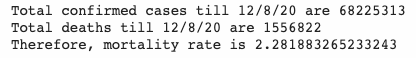
\includegraphics[scale=0.5]{stats}
\end{figure}

\end{frame}

\begin{frame}{Problem Statement}
To contain the spread of the virus, it is extremely important to deploy technology for its future trends.\\

\medskip

Tracking the active corona cases as they crop up helps governments and common people be cautious about their future plans. They may then decide and form policies for better control over the virus. It will lead to less havoc and lower fatality rate.

\medskip

In this project, we aim to develop a probabilistic predictor for confirmed coronavirus cases in future 1 to 30 day window. Our objective is to correlate this prediction with the GDP projection in that particular region.
\end{frame}

\begin{frame}{Literature}
The SIR family of models are among the most popular ones to learn the dynamics of COVID-19. The SIRD model is an extension of the SIR model, and is used to demonstrate the differences of infectious rate at different countries.\\

There are models available based on Markov chain Monte Carlo methods and other kinds of Bayes filters like Particle filters and Kalman filters.
\end{frame}

\begin{frame}{Dataset}
\begin{itemize}
\item All reported experiments are based on online COVID-19 data repository maintained by John Hopkins University - \url{https://github.com/CSSEGISandData/COVID-19} - for time-period of 22 January 2020 to 8 December 2020.
\item Dataset for GDP Projection:
\footnote{links for dataset on last slide}
\begin{itemize}
\item Gross Domestic Product(Real Index) - IMF Data 
\item Total Population (2019) (Worldbank) 
\item Unemployment (Worldbank) 
\item Unemployment [FOR INDIA] 
\item Mobile cellular subscriptions (Worldbank)
\item Population age 65 and above data (Worldbank) 
\end{itemize}
\end{itemize}
\end{frame}

\begin{frame}{Methodology}
\begin{itemize}
\item The dataset was filtered and structured.
\item Time-series analysis of data to decipher trends.
\item  An adaptive online Kalman filter provides us a very good one-day prediction for each region.
\item It was extended for a window of 30 days which showed how Kalman filter behaves undesirably for long-term predictions.
\item The results of this predictor are used in projecting the GDP of a region.
\end{itemize}

\end{frame}

\begin{frame}{Data Preprocessing}
\begin{itemize}
\item Read the data containing daily total cases of confirmed, death and recovered.
\item Fix region names.
\item Consider regions for which reliable population data is available.
\item Missing values are handled using interpolation.
\item Data was scaled quarter-wise from the available annual data using interpolation.
\end{itemize}
\end{frame}

\begin{frame}{Visualisations}
\begin{figure}[!h]
\begin{subfigure}{.5\textwidth}
\centering
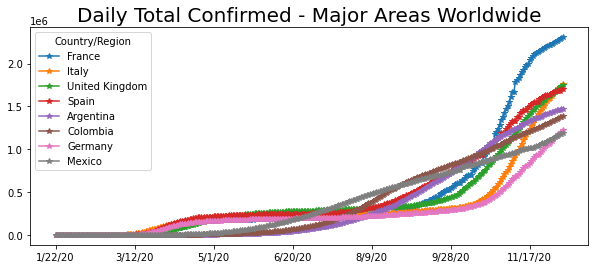
\includegraphics[width=1\linewidth]{conf.png}
\end{subfigure}%
\begin{subfigure}{.5\textwidth}
\centering
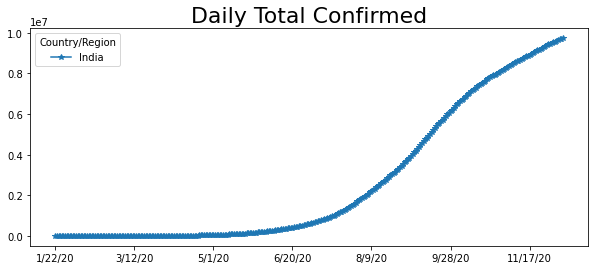
\includegraphics[width=1\linewidth]{india_conf.png}
\end{subfigure}
\end{figure}
We can see a steep growth of active cases in India from July as the lockdown was lifted.
\end{frame}

\begin{frame}{Kalman Filters}
Kalman filter (KF) is a widely used method for tracking and navigation, and for filtering and prediction of econometric time series data. Kalman filter is a recursive algorithm that uses time-series measurement over time, containing statistical noise and produce estimations of unknown variables.

\medskip

Each day the algorithm needs to be updated with new observation, after the estimation is done it can generate predictions for the next day.

\medskip

No overfitting or bias as it is an online algorithm.

\medskip

Error function : RMSE and MAE
\end{frame}

\begin{frame}{Features}
\begin{itemize}
\item Confirmed cases
\item One day change
\item Three day change
\item Five day change
\item Seven day change
\item One day change rate (100*(One day change) / (Cases 1 day ago))
\item Three day change rate
\item Five day change rate
\item Seven day change rate
\item Infected rate
\item Kalman Prediction
\end{itemize}
\end{frame}


\begin{frame}{Results}
Training Date - 22 January, 2020 to 7 December, 2020 \\
Testing Date - 8 December 2020 to 9 December, 2020
\begin{figure}
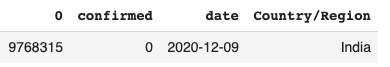
\includegraphics[scale=0.5]{kal_1day}
\caption{1-Day Prediction  for Confirmed Cases, India}
\end{figure}

\begin{center}
Actual cases on 2020-12-09 in India = 9771292
\end{center}
\end{frame}

\begin{frame}{Results}
\begin{figure}
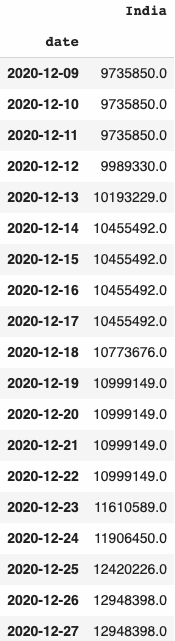
\includegraphics[scale=0.3]{kal_30day}
\caption{30-day Prediction Table for Confirmed Cases, India}
\end{figure}
\end{frame}

\begin{frame}{Results}
\begin{figure}
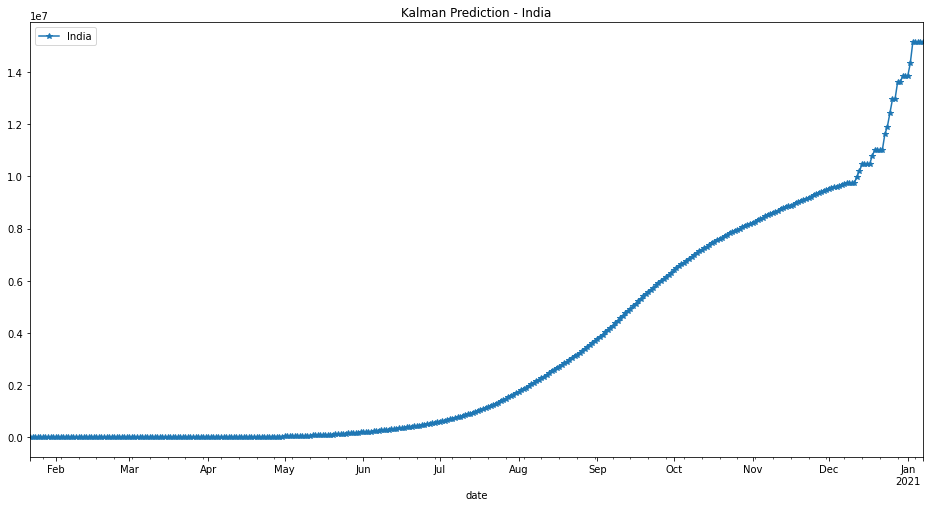
\includegraphics[scale=0.35]{30day_kal}
\caption{Prediction Curve for India (Long-term)}
\end{figure}
\end{frame}

\begin{frame}{Results}
\begin{figure}
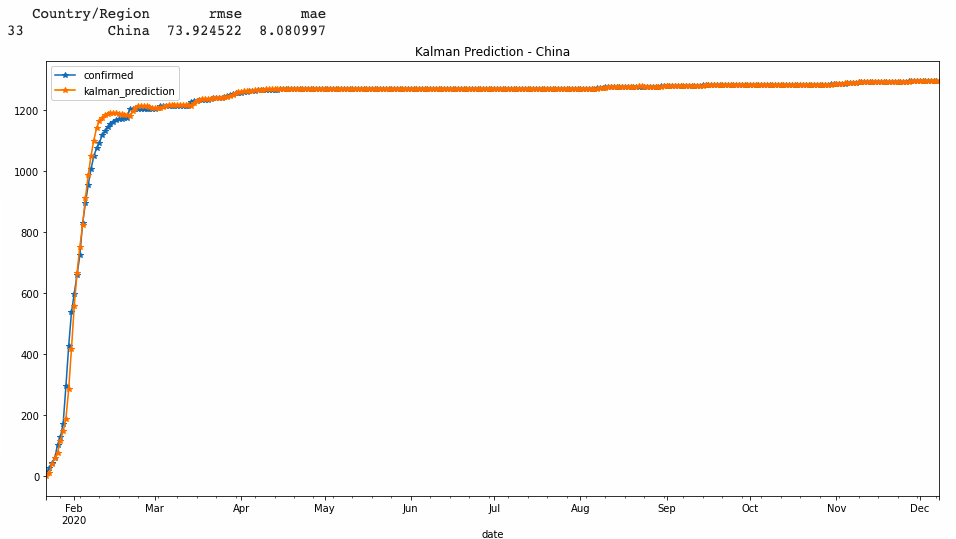
\includegraphics[scale=0.3]{kal_china}
\caption{Prediction Curve for China (Short-term)}
\end{figure}
\end{frame}


\begin{frame}{Neural Net}
\textbf{Architecture}
\begin{itemize}
\item An input layer, 3 hidden layers, An output layer
\item Activation function - LeakyRELU
\item Optimizer - Adam
\item Learning Rate - 0.001
\item Cost function - MSE
\end{itemize}
\end{frame}
\begin{frame}{Results}
\begin{figure}
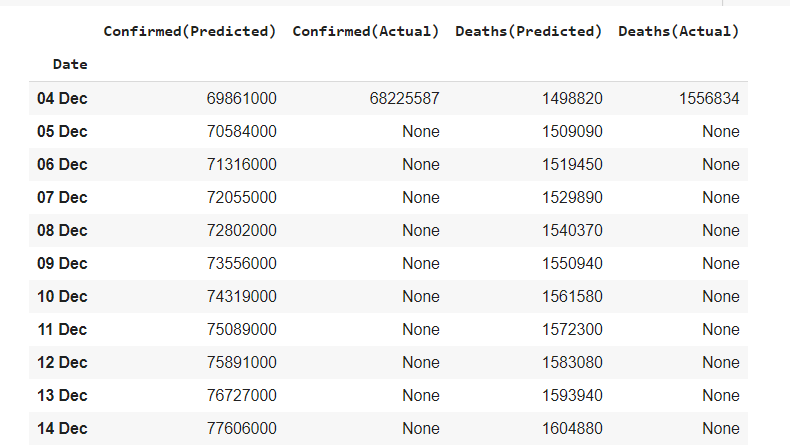
\includegraphics[scale=0.7]{neural_net_pred}
\caption{Prediction Table for Global Confirmed and Death Cases}
\end{figure}
\end{frame}

\begin{frame}{Results}
\begin{figure}
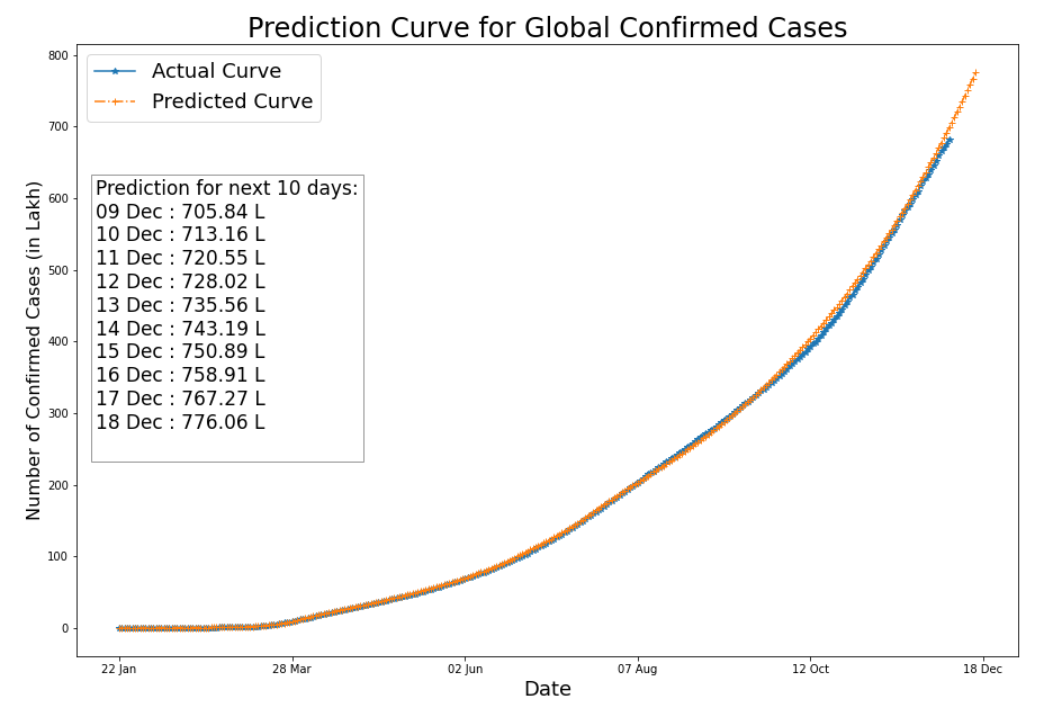
\includegraphics[scale=0.45]{neural_confirm_pred}
\caption{Prediction Curve for Global Confirmed Cases}
\end{figure}
\end{frame}

\begin{frame}{Results}
\begin{figure}
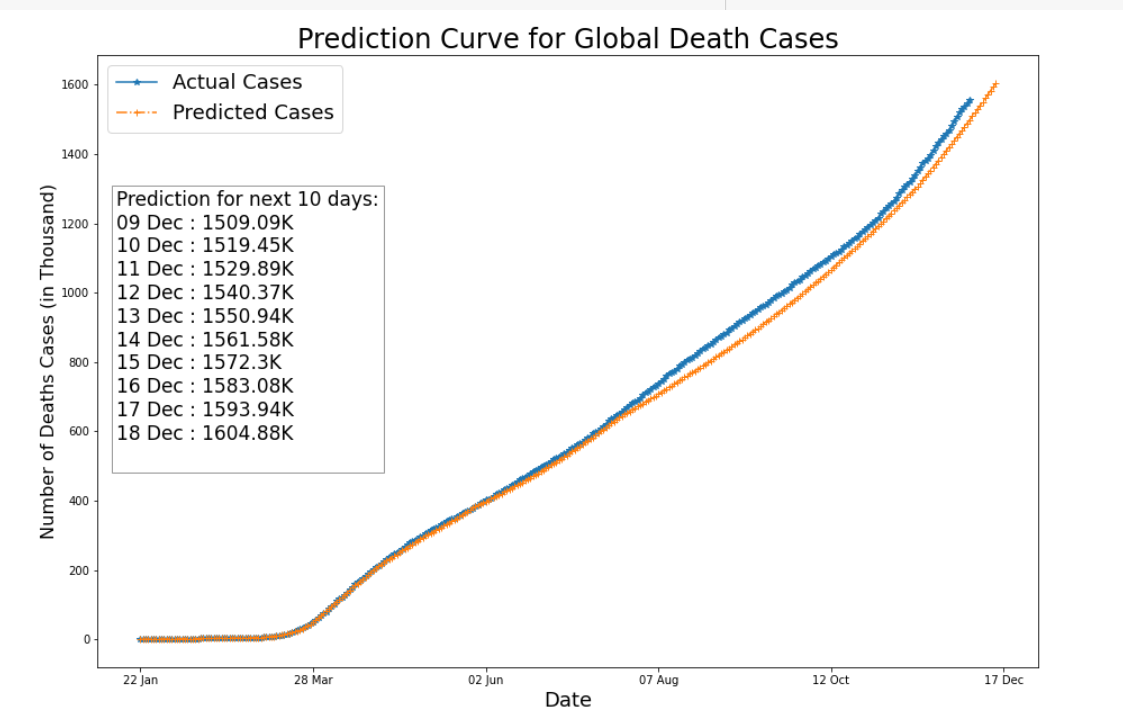
\includegraphics[scale=0.45]{neural_death_pred}
\caption{Prediction Curve for Global Death Cases}
\end{figure}
\end{frame}
\begin{frame}{GDP Predictor}
\textbf{Features used for training the model}
\begin{itemize}
\item Total Population
\item Unemployment Ratio
\item Mobile cellular subscriptions
\item Population above 65 years of age
\item Predicted COVID-19 cases (for 2020 Quarter 3)
\end{itemize}
\end{frame}

\begin{frame}{Random Forest Regressor}
\begin{itemize}
\item Ensemble learning method for classification
\item Can be used for regression too
\item Constructs several DTs at training time
\item Outputs mean of individual trees
\item Hyperparameters: Estimators = 4 , Criterion : MSE
\end{itemize}
\end{frame}



\begin{frame}{Flowchart for GDP Prediction}
\begin{figure}
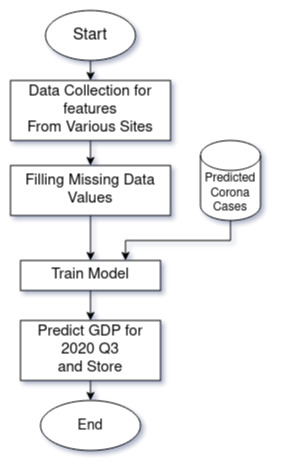
\includegraphics[scale=0.4]{ml_image_io.jpg}

\end{figure}
\end{frame}


\begin{frame}{Results}
\begin{figure}
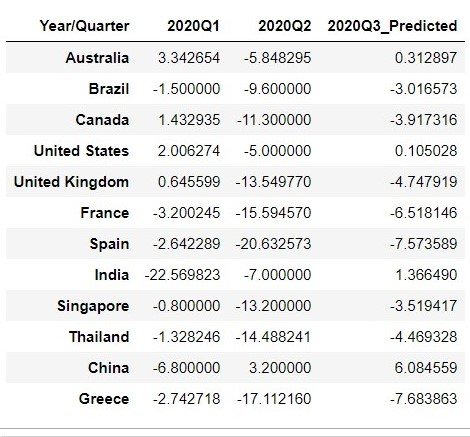
\includegraphics[scale=0.7]{gdp_prediction.jpeg}
\caption{Prediction of percent change in GDP of Countries}
\end{figure}
\end{frame}

\begin{frame}{Discussion}
\begin{itemize}
\item Population and daily total confirmed cases are used to calculate the infected rate of each area (in percentage).
\item Kalman prediction and time-dependent variables like day-wise changes are correlated to the target i.e. confirmed cases.
\item The 1-day Kalman prediction is very accurate and powerful while a longer period prediction is more challenging but provides a future trend.
\item Large mean average error for longer predictions.
\item Historical data has less effect on prediction as compared to the previous day data.
\item GDP projection is somewhat consistent with actual projections for countries that provided comprehensive data about the influencers.
\end{itemize}
\end{frame}


\begin{frame}{Future Work}
\begin{itemize}
    \item Take testing scale into account.
    \item Correlate the predictions with other factors like healthcare, age groups etc.
    \item Continuous evaluation of GDP instead of quaterly evaluation.
\end{itemize}

\end{frame}

\begin{frame}{External Links}
\begin{itemize}
\item Gross Domestic Product(Real Index) - \url{https://data.imf.org/?sk=4c514d48-b6ba-49ed-8ab9-52b0c1a0179b}
\item Total Population (2019) - \url{api.worldbank.org/v2/en/indicator/SP.POP.TOTL?downloadformat=csv}
\item Unemployment - \url{api.worldbank.org/v2/en/indicator/SL.UEM.TOTL.ZS?downloadformat=csv}
\item Unemployment [FOR INDIA] - \url{https://www.macrotrends.net/countries/IND/india/unemployment-rate}
\item Mobile cellular subscriptions - \url{api.worldbank.org/v2/en/indicator/IT.CEL.SETS.P2?downloadformat=csv}
\item Population age 65 and above data - \url{api.worldbank.org/v2/en/indicator/SP.POP.65UP.TO.ZS?downloadformat=csv}
\end{itemize}
\end{frame}

\begin{frame}{References}
    \url{https://link.springer.com/article/10.1007/s10489-020-01948-1}
\end{frame}
\begin{frame}
\center \textbf{THANK YOU}
    
\end{frame}
\end{document}